\title{Self Organizing Systems Exercise 3}
\author{
        Alexander Dobler 01631858\\
        Thomas Kaufmann 01129115 
}
\date{\today}

\documentclass[12pt]{article}

\usepackage{hyperref}
\usepackage{booktabs}
\usepackage{graphics}
\usepackage{multirow}
\usepackage{graphicx}
\usepackage{subcaption}
\usepackage{mwe}
\usepackage{amsmath,amssymb}
\usepackage{subcaption}
\usepackage[section]{placeins}

\begin{document}
\maketitle

\section{Implementation}
\paragraph*{Explanation of the Implementation}
The implementation is described directly in the jupyter notebook.
We implemented the k-NN-based and the radius-based neighborhood graphs.
Both implementations can be found in the \textit{SomViz} class under the methods \textit{neighbourhood\_knn} and \textit{neighbourhood\_radius}.

\paragraph*{Adapting Parameters}
Adapting parameters is as easy as changing the parameter \textit{k} for the function \textit{neighbourhood\_knn} and the parameter \textit{radius} for \textit{neighbourhood\_radius}.
We provide a section for each dataset, so one can try out different parameters for every dataset.

\section{Evaluation}
The neighborhood visualisations are projected onto the U-matrix visualisations.
\paragraph*{Chainlink Dataset}
\begin{figure}[t]
    \centering
    \begin{subfigure}{.5\textwidth}
      \centering
      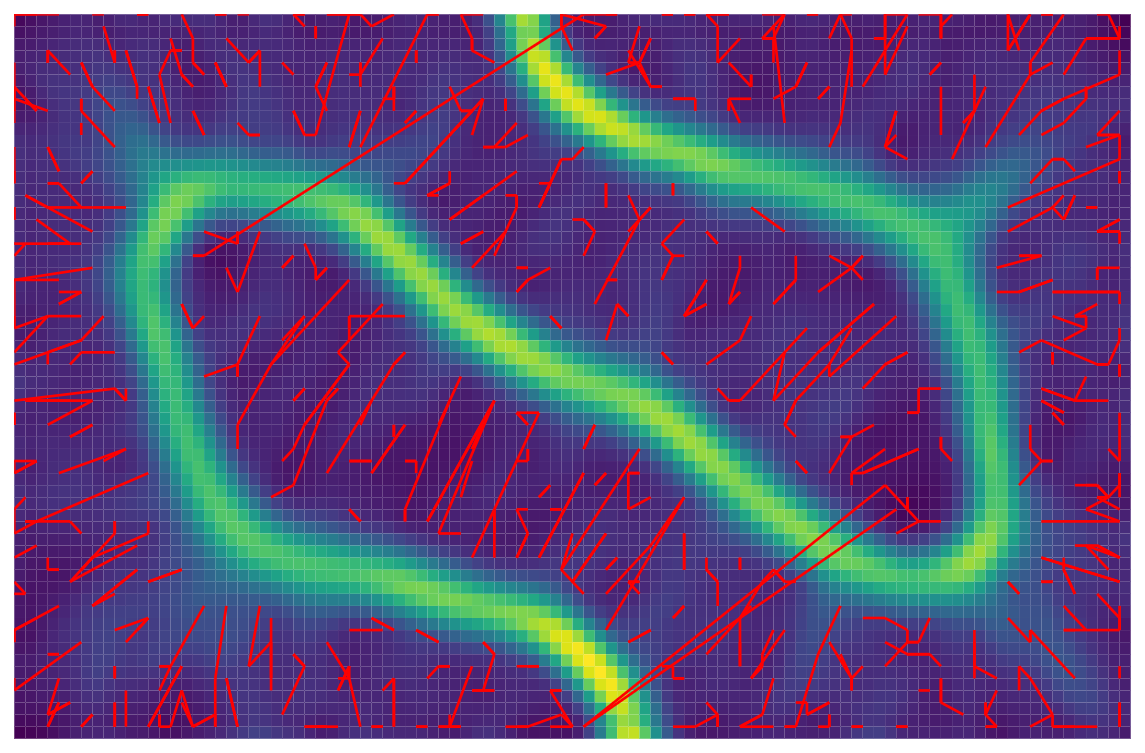
\includegraphics[width=.9\linewidth]{vis/chainlink_k_1.png}
      \caption{$k=1$}
      \label{fig:chainlinkk1}
    \end{subfigure}%
    \begin{subfigure}{.5\textwidth}
      \centering
      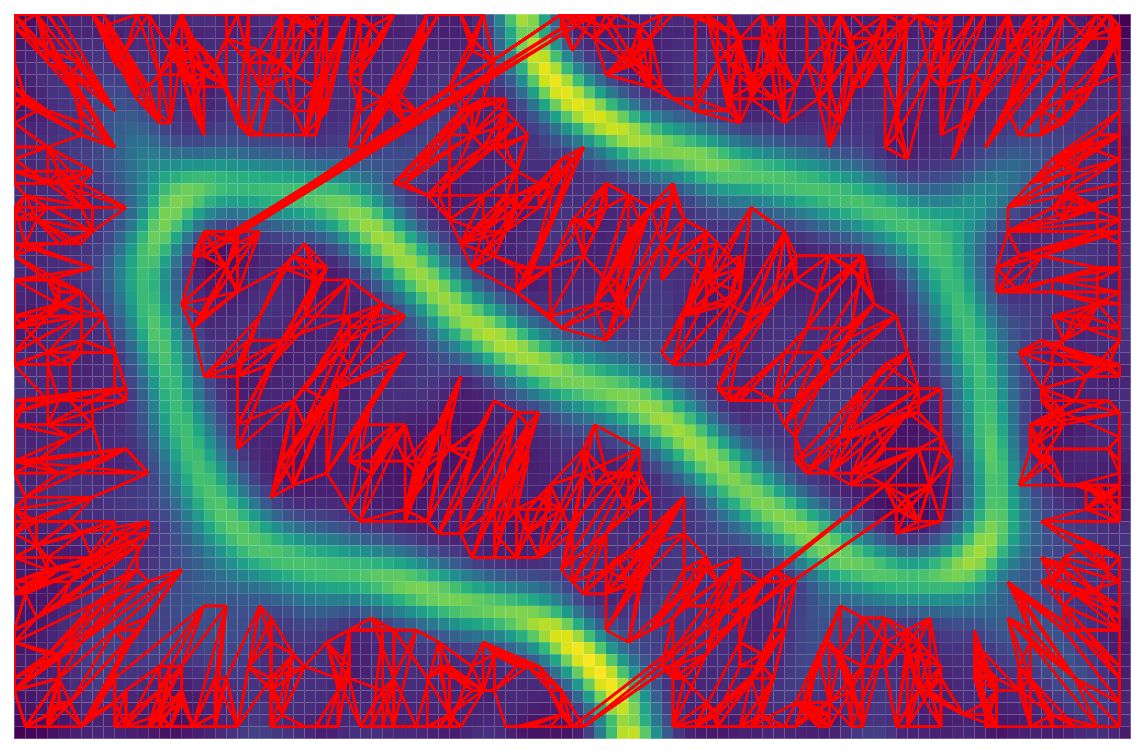
\includegraphics[width=.9\linewidth]{vis/chainlink_k_5.png}
      \caption{$k=5$}
      \label{fig:chainlinkk5}
    \end{subfigure}
    \caption{Chainlink dataset: K-NN visualisations}
    \label{fig:chainlinkknn}
\end{figure}
\begin{figure}[t]
    \centering
    \begin{subfigure}{.5\textwidth}
        \centering
        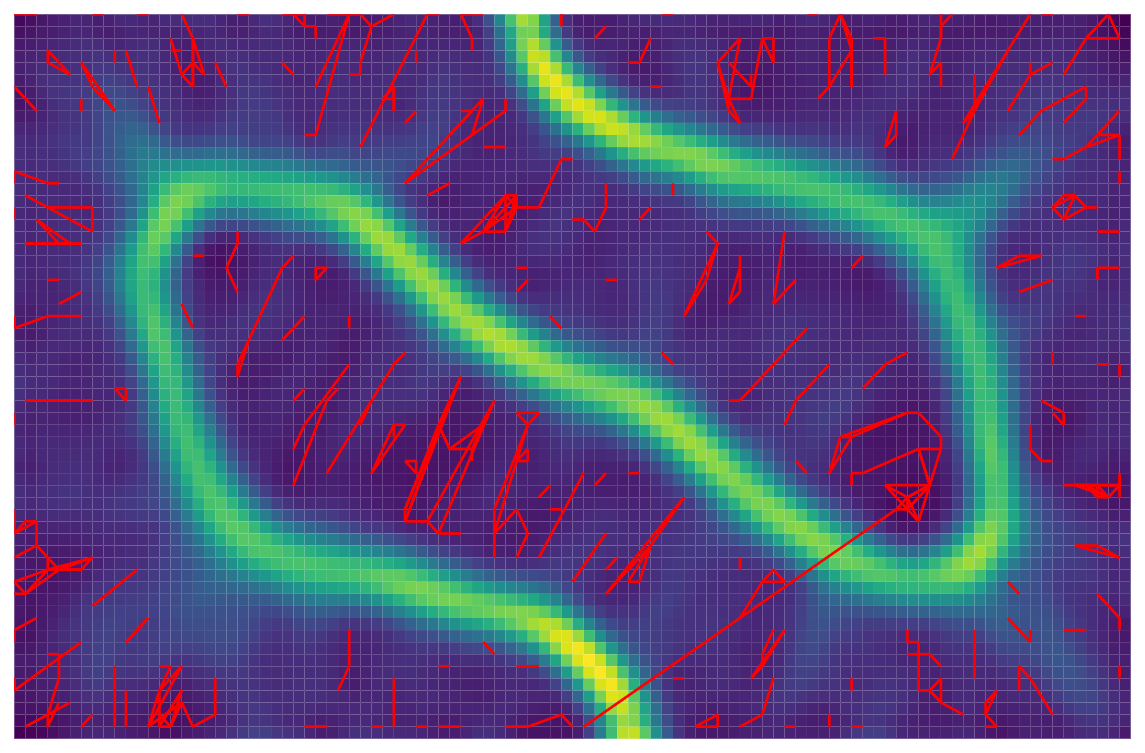
\includegraphics[width=.9\linewidth]{vis/chainlink_r_005.png}
        \caption{$r=0.05$}
        \label{fig:chainlinkr0.05}
    \end{subfigure}%
    \begin{subfigure}{.5\textwidth}
        \centering
        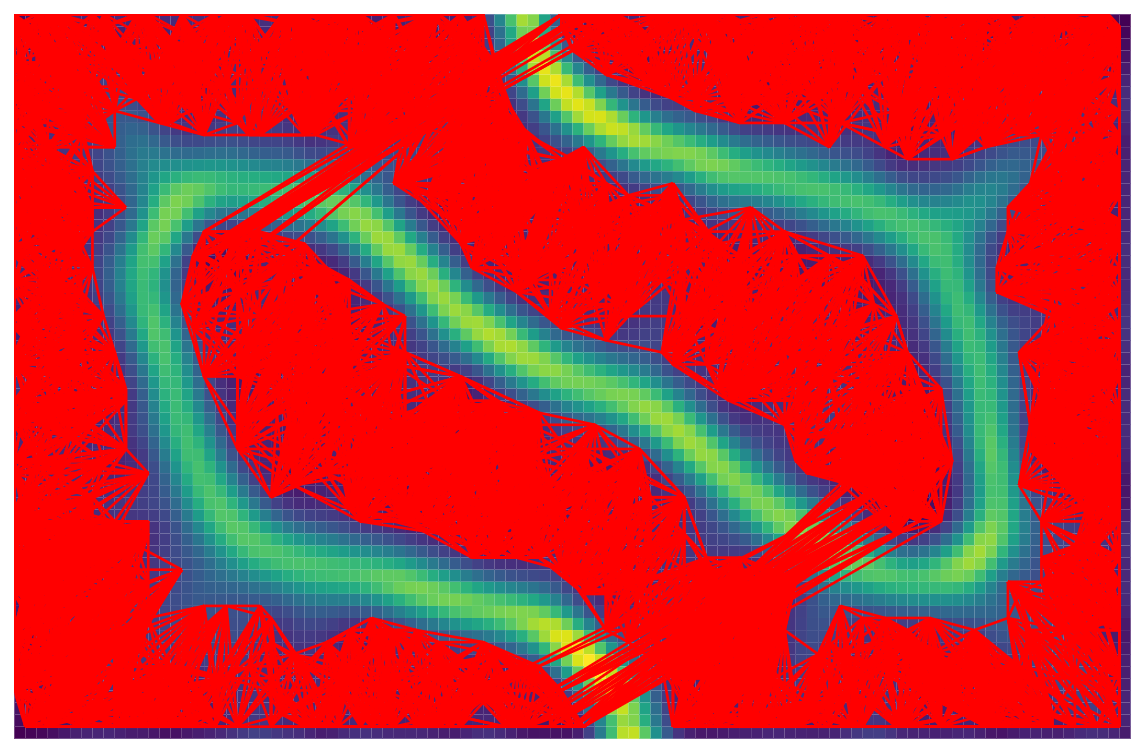
\includegraphics[width=.9\linewidth]{vis/chainlink_r_02.png}
        \caption{$r=0.2$}
        \label{fig:chainlinkr0.2}
    \end{subfigure}
    \caption{Chainlink dataset: Radius-based visualisations}
    \label{fig:chainlinkradius}
\end{figure}
In Figure~\ref{fig:chainlinkknn} and Figure~\ref{fig:chainlinkradius} we can see the created visualisations for the chainlink data set for different parameters.
The induced topology violations are clearly visible by the connections crossing the green interpolating aray.
We can also see, how the parameter settings change the visualisations:
Increasing the parameter $k$ for the k-NN based neighborhood graph and the radius for the radius-based neighborhood graphs increases the number of connections between units.
Setting the radius to a high value, we get somewhat of a connected red region, resembling cluster structures.

Obviously both visualisations can be used to identify density information and topology violations.

\paragraph*{10 Clusters Dataset}
\begin{figure}[t]
    \centering
    \begin{subfigure}{.5\textwidth}
      \centering
      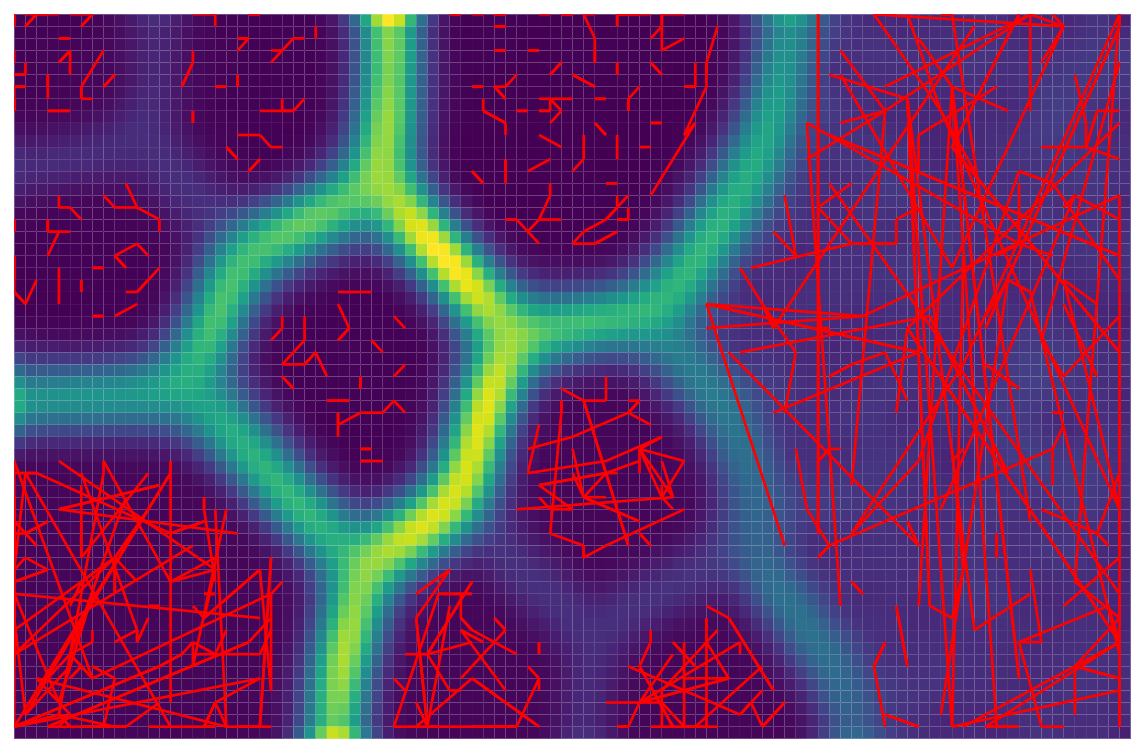
\includegraphics[width=.9\linewidth]{vis/10clusters_k_1.png}
      \caption{$k=1$}
      \label{fig:10clustersk1}
    \end{subfigure}%
    \begin{subfigure}{.5\textwidth}
      \centering
      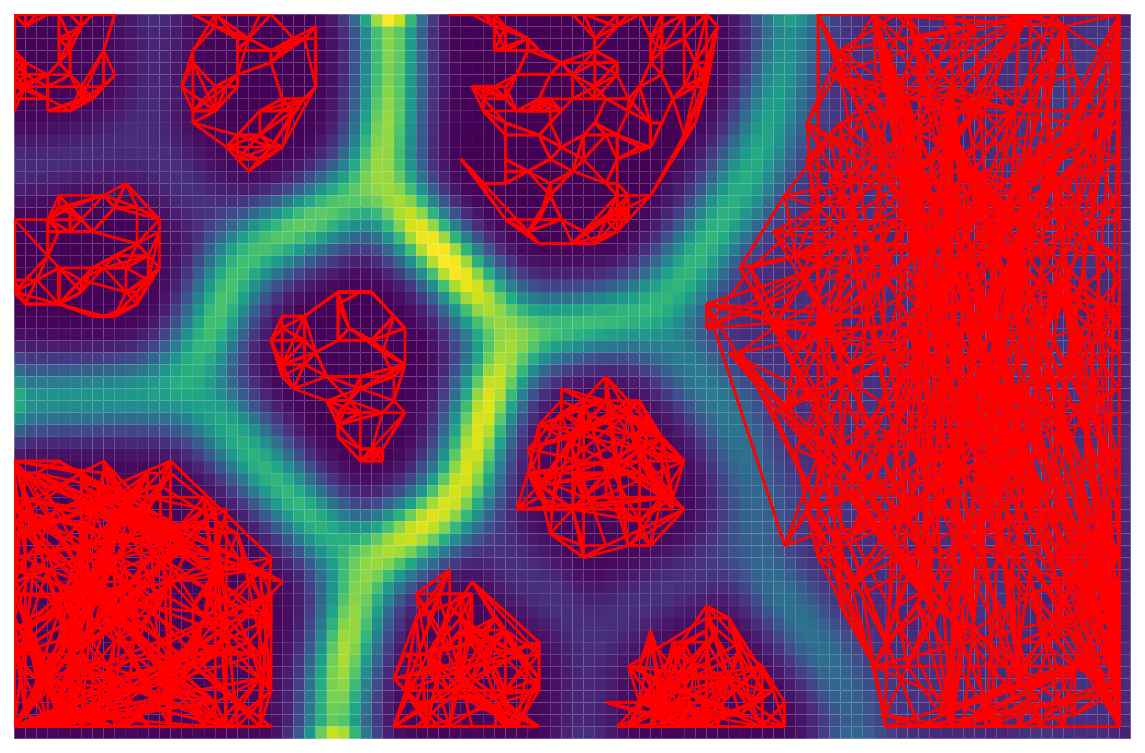
\includegraphics[width=.9\linewidth]{vis/10clusters_k_5.png}
      \caption{$k=5$}
      \label{fig:10clustersk5}
    \end{subfigure}
    \caption{10 clusters dataset: K-NN visualisations}
    \label{fig:10clustersknn}
\end{figure}
\begin{figure}[t]
    \centering
    \begin{subfigure}{.5\textwidth}
        \centering
        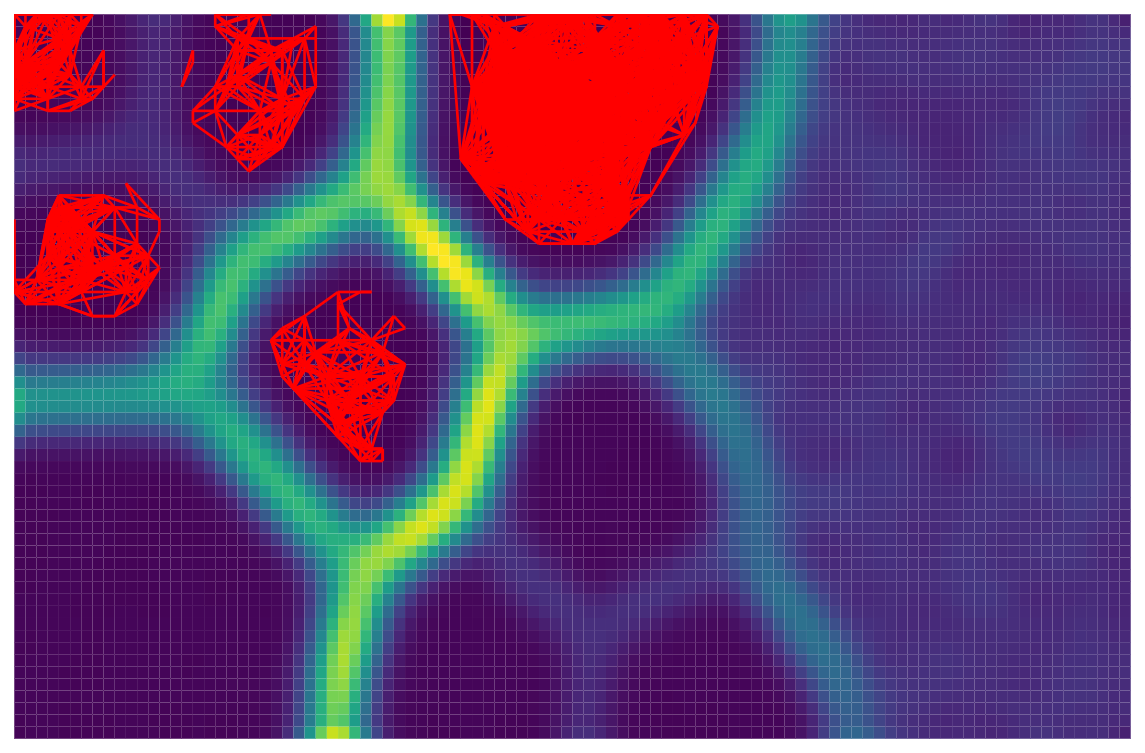
\includegraphics[width=.9\linewidth]{vis/10clusters_r_01.png}
        \caption{$r=0.1$}
        \label{fig:chainlinkr0.1}
    \end{subfigure}%
    \begin{subfigure}{.5\textwidth}
        \centering
        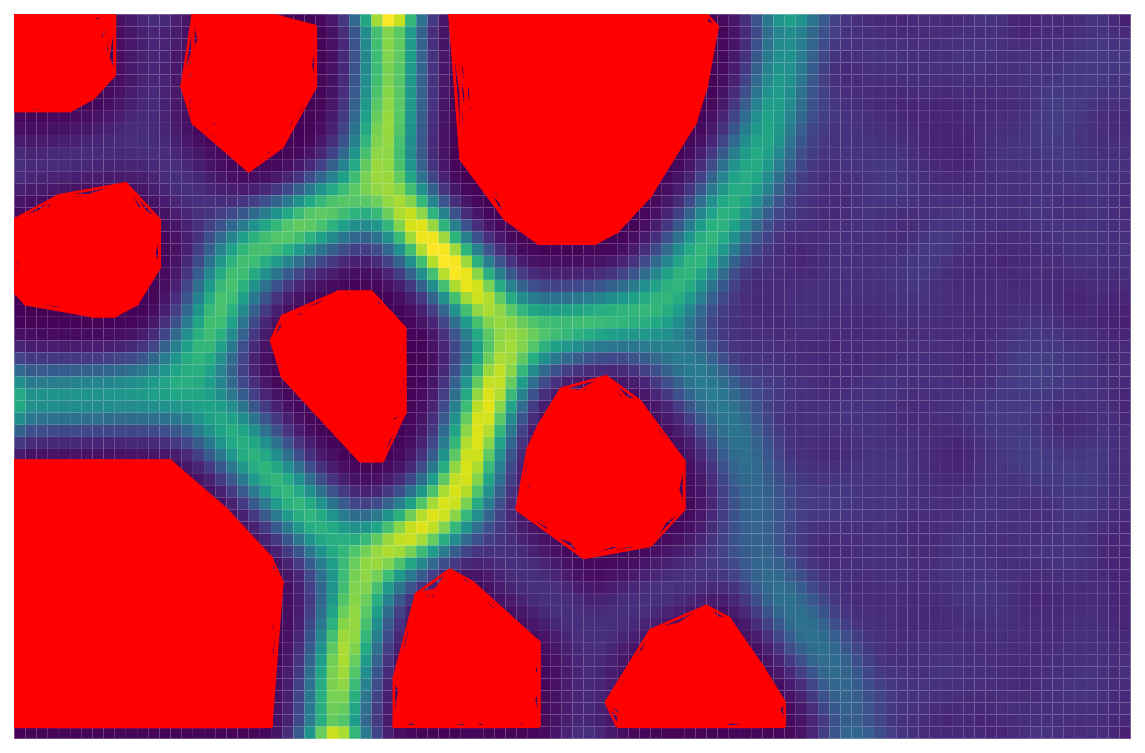
\includegraphics[width=.9\linewidth]{vis/10clusters_r_1.png}
        \caption{$r=1$}
        \label{fig:chainlinkr1}
    \end{subfigure}
    \caption{10 clusters dataset: Radius-based visualisations}
    \label{fig:10clustersradius}
\end{figure}
In Figure~\ref{fig:10clustersknn} and Figure~\ref{fig:10clustersradius} we can see the k-NN based and radius-based neighborhood graphs for the 10 clusters dataset projected onto the U-matrix visualisation.
While the k-NN based neighborhood graph detects all 10 clusters, the radius-based neighborhood does not detect the clusters with big standard deviation to the right.
Both visualisations clearly show density information:
The k-NN based neighborhood graph detects all 10 clusters, while the radius-based neighborhood graph detects how \textit{dense} these clusters themselfs are.

\section{Comparison with SOM Toolbox}
\begin{figure}[t]
    \centering
    \begin{subfigure}{.5\textwidth}
      \centering
      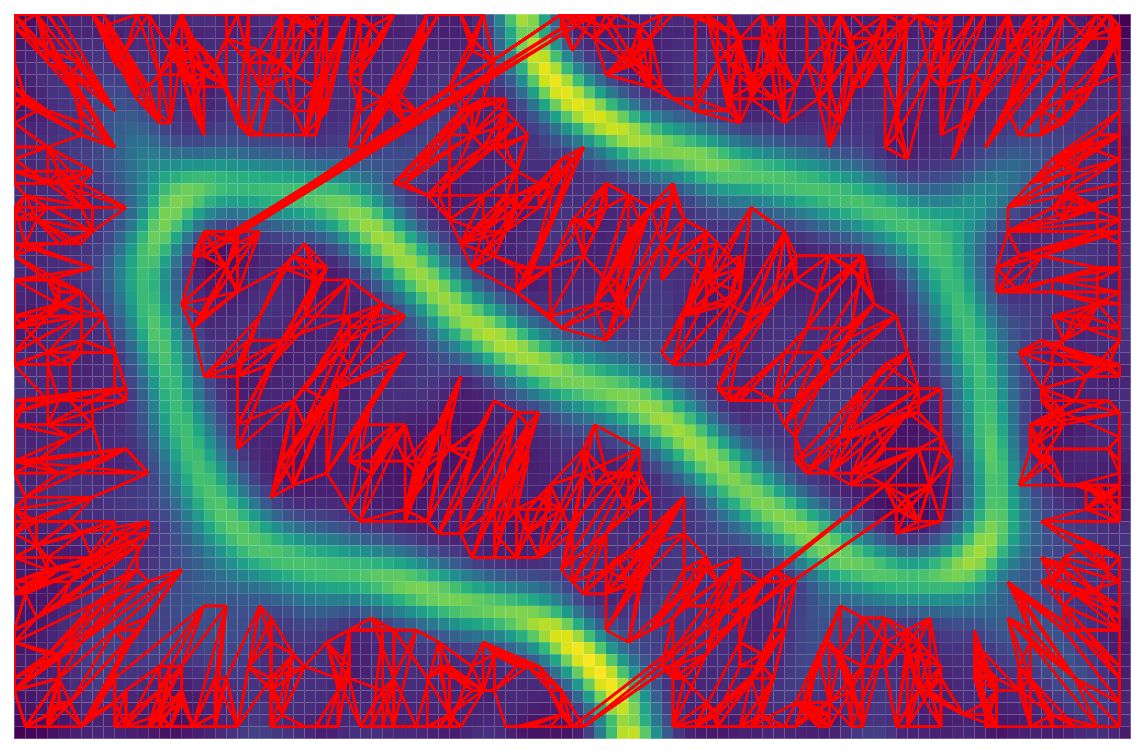
\includegraphics[width=.9\linewidth]{vis/chainlink_k_5.png}
      \caption{Implementation}
    \end{subfigure}%
    \begin{subfigure}{.5\textwidth}
      \centering
      \includegraphics[width=.9\linewidth]{vis/chainlink_k_5_somtoolbox.png}
      \caption{SOM toolbox}
    \end{subfigure}
    \caption{Chainlink dataset: K-NN comparison}
    \label{fig:chainlinkknncomparison}
\end{figure}
\begin{figure}[t]
    \centering
    \begin{subfigure}{.5\textwidth}
        \centering
        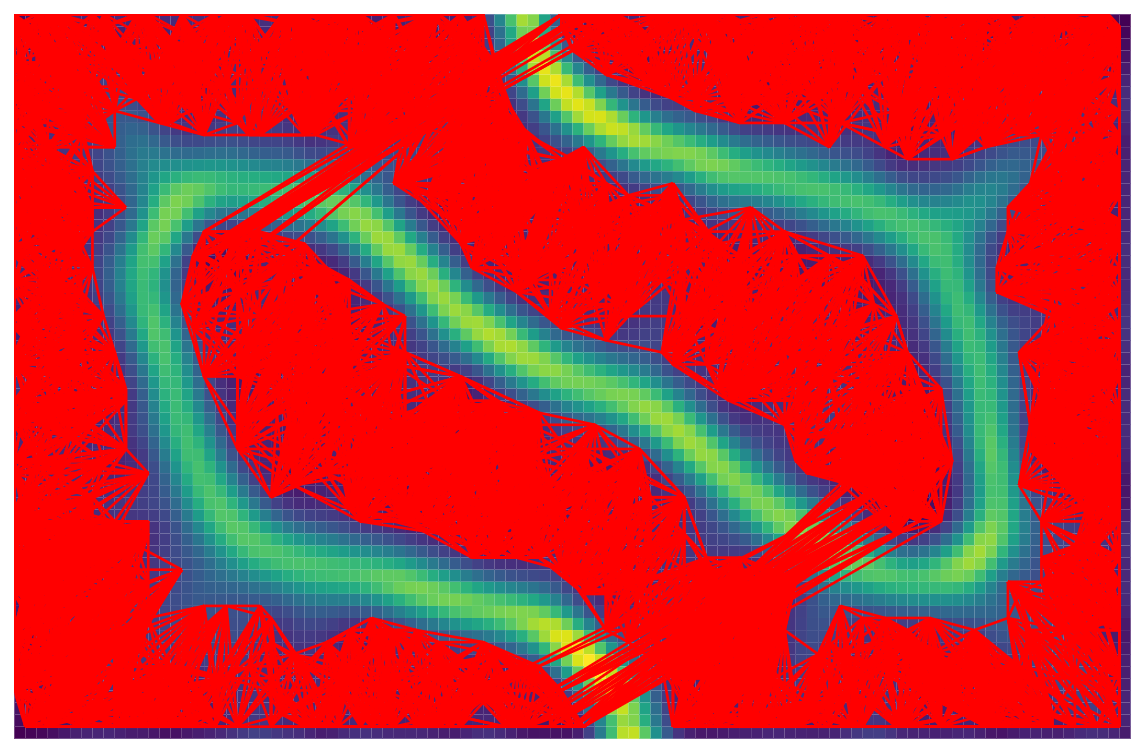
\includegraphics[width=.9\linewidth]{vis/chainlink_r_02.png}
        \caption{Implementation}
    \end{subfigure}%
    \begin{subfigure}{.5\textwidth}
        \centering
        \includegraphics[width=.9\linewidth]{vis/chainlink_r_02_somtoolbox.png}
        \caption{SOM toolbox}
    \end{subfigure}
    \caption{Chainlink dataset: Radius-based comparison}
    \label{fig:chainlinkradiuscomparison}
\end{figure}
\begin{figure}[t]
    \centering
    \begin{subfigure}{.5\textwidth}
      \centering
      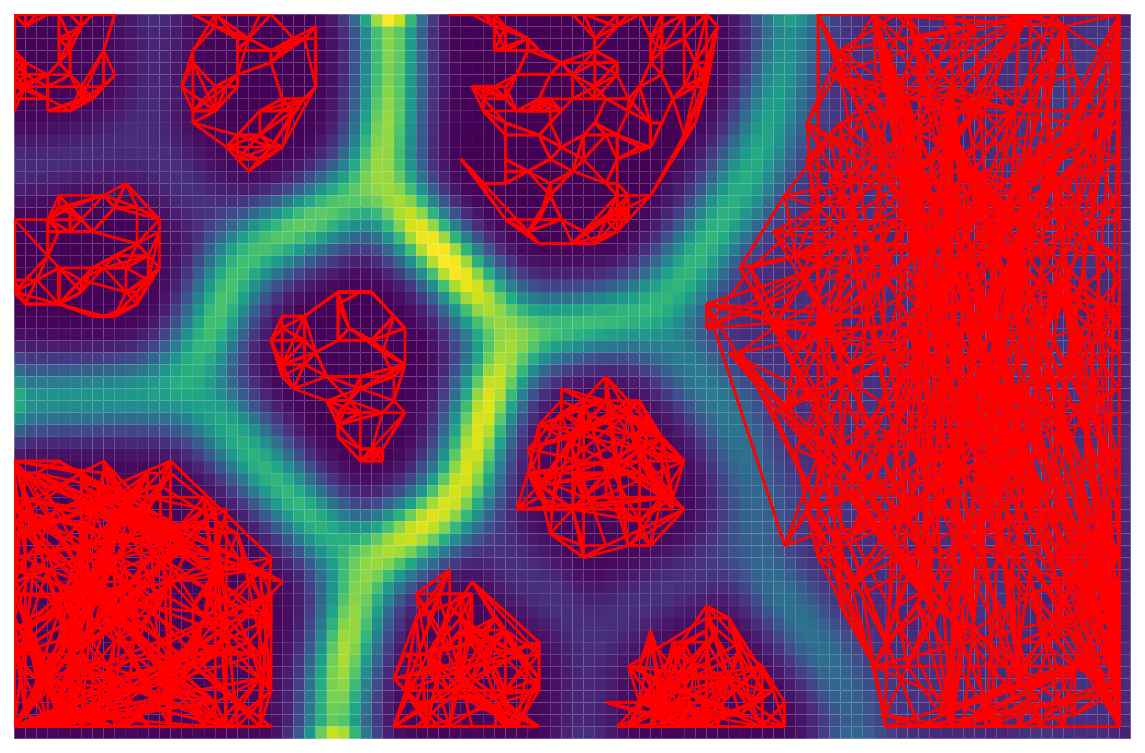
\includegraphics[width=.9\linewidth]{vis/10clusters_k_5.png}
      \caption{Implementation}
    \end{subfigure}%
    \begin{subfigure}{.5\textwidth}
      \centering
      \includegraphics[width=.9\linewidth]{vis/10clusters_k_5_somtoolbox.png}
      \caption{SOM toolbox}
    \end{subfigure}
    \caption{10 clusters dataset: K-NN comparison}
    \label{fig:10clustersknncomparison}
\end{figure}
\begin{figure}[t]
    \centering
    \begin{subfigure}{.5\textwidth}
        \centering
        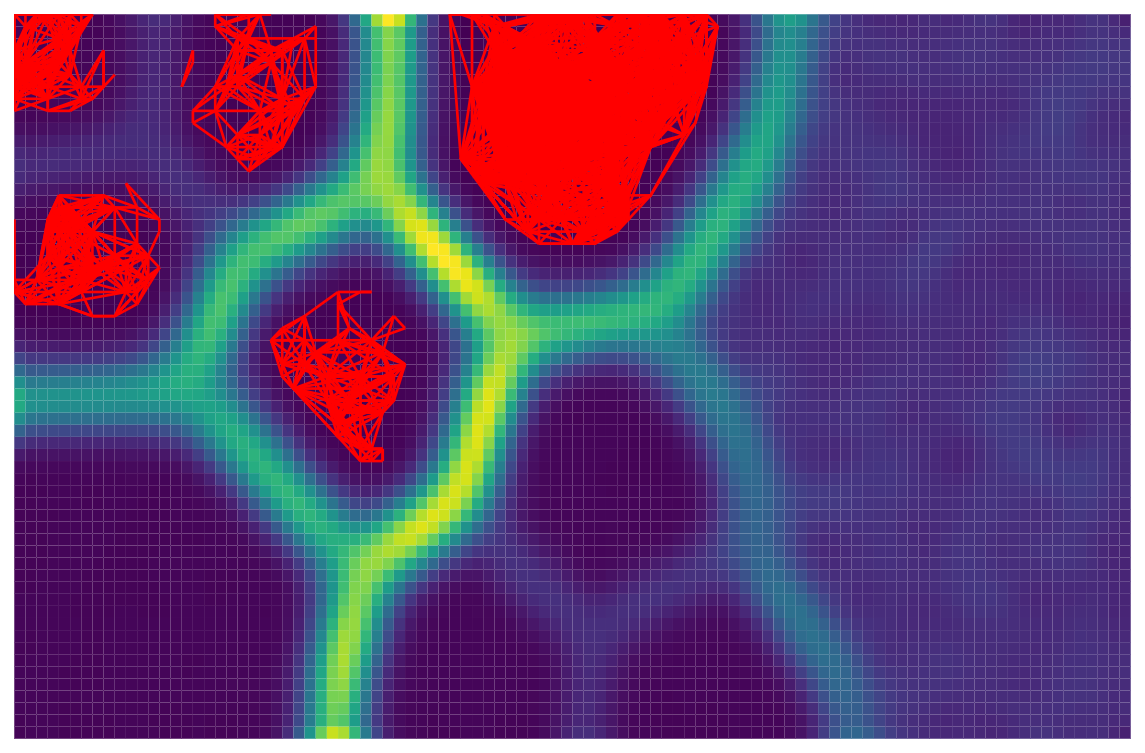
\includegraphics[width=.9\linewidth]{vis/10clusters_r_01.png}
        \caption{Implementation}
    \end{subfigure}%
    \begin{subfigure}{.5\textwidth}
        \centering
        \includegraphics[width=.9\linewidth]{vis/10clusters_r_01_somtoolbox.png}
        \caption{SOM Toolbox}
    \end{subfigure}
    \caption{10 clusters dataset: Radius-based comparison}
    \label{fig:10clustersradiuscomparison}
\end{figure}
In Figures~\ref{fig:chainlinkknncomparison}-\ref{fig:10clustersradiuscomparison} we can see the comparison between visualisations generated by our implementation and the ones generated by SOM toolbox.
Clearly they are identical, which means our implementation is correct.

\section{Conclusion}
Having the weight and input vector files, generating the neighborhood graph is easy when using for example KD-trees for computing nearest neighbors.
\end{document}
  